% Chương 1: Tổng quan đề tài

\chapter{Tổng quan đề tài}

\label{Chapter1}

\newcommand{\keyword}[1]{\textbf{#1}}
\newcommand{\tabhead}[1]{\textbf{#1}}
\newcommand{\code}[1]{\texttt{#1}}
\newcommand{\file}[1]{\texttt{\bfseries#1}}
\newcommand{\option}[1]{\texttt{\itshape#1}}

%----------------------------------------------------------------------------------------

\section{Bối cảnh và động lực nghiên cứu}

U não là nhóm bệnh lý ác tính có tỷ lệ tử vong cao và diễn tiến nhanh. U thần kinh đệm độ cao (glioblastoma multiforme, GBM) có trung vị thời gian sống sau chẩn đoán chỉ khoảng 14--16 tháng ngay cả khi được phẫu thuật, xạ trị và hóa trị kết hợp \cite{Menze2015}. Ở nhóm u thần kinh đệm độ thấp (LGG), tiên lượng khả quan hơn song bệnh nhân vẫn đối mặt với nguy cơ tiến triển sang thể ác tính cao. Thời điểm phát hiện bệnh đóng vai trò then chốt: u được chẩn đoán ở giai đoạn sớm, khi kích thước còn nhỏ và chưa xâm lấn các cấu trúc quan trọng, cho phép can thiệp triệt để hơn và cải thiện tiên lượng đáng kể.

Ảnh cộng hưởng từ (MRI) là phương tiện hình ảnh học được lựa chọn hàng đầu để đánh giá bệnh lý não bộ nhờ độ tương phản mô mềm vượt trội so với CT và khả năng hiển thị rõ ranh giới khối u. Một nghiên cứu MRI não điển hình có thể bao gồm hàng chục đến hàng trăm lát cắt với nhiều chuỗi xung khác nhau (T1, T2, FLAIR, T1 tăng cường tương phản), tạo ra khối lượng dữ liệu đáng kể cần được bác sĩ chẩn đoán hình ảnh phân tích thủ công. Với khối lượng công việc thủ công lớn, cùng với sự thiếu hụt nhân lực chuyên khoa tại nhiều cơ sở y tế, đặc biệt ở các nước đang phát triển, tạo ra nhu cầu cấp thiết về công cụ hỗ trợ chẩn đoán tự động.

Các mô hình học sâu và đặc biệt là các mạng nơ-ron tích chập (CNN) đã chứng minh hiệu quả vượt trội trong các bài toán phân tích ảnh y tế \cite{Litjens2017}. Tuy nhiên, một thách thức cơ bản khi triển khai các mô hình học sâu trong lâm sàng là vấn đề ``hộp đen'' (black box): mô hình đưa ra kết quả nhưng không cung cấp giải thích về cơ sở của quyết định. Bác sĩ lâm sàng cần hiểu \textit{tại sao} hệ thống AI đánh dấu một vùng là khối u, chứ không chỉ biết rằng nó là khối u. Đây là điều kiện tiên quyết để AI có thể được chấp nhận và tin tưởng trong thực hành y tế \cite{Doshi2017}.

\begin{figure}[h!]
    \centering
    \subfigure[Ảnh MRI não (T1-Gd, axial)]{
        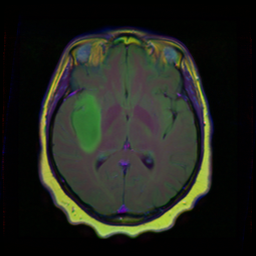
\includegraphics[width=0.30\textwidth]{Figures/Gallery/BrainMRI.png}
    }
    \hspace{4pt}
    \subfigure[Mặt nạ phân đoạn (ground truth)]{
        
\includegraphics[width=0.30\textwidth]{Figures/Gallery/Tumor_Mask.png}
    }
    \hspace{4pt}
    \subfigure[Overlay: vùng khối u (xanh lá)]{
        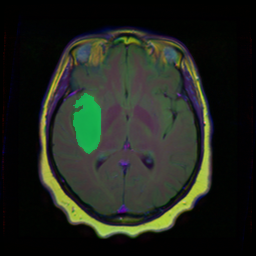
\includegraphics[width=0.30\textwidth]{Figures/Gallery/BrainMRI_overlay.png}
    }
    \caption{Ví dụ một mẫu từ bộ dữ liệu LGG MRI Segmentation \cite{Buda2019}: ảnh MRI gốc (trái), mặt nạ nhị phân do chuyên gia chú thích (giữa) và overlay vùng khối u trên ảnh gốc (phải). Đây là định dạng đầu vào và đầu ra của bài toán phân đoạn tự động.}
    \label{fig:mri_example}
\end{figure}

\section{Tổng quan bài toán}

Bài toán nghiên cứu được xác định như sau:

\textbf{Đầu vào:} Một ảnh MRI não dạng 2D (một lát cắt đơn), định dạng JPEG hoặc PNG, kích thước tùy ý.

\textbf{Yêu cầu xử lý:}
\begin{enumerate}
    \item \textit{Phân đoạn tự động:} Tạo ra mặt nạ nhị phân ($256 \times 256$ pixel) xác định các pixel thuộc vùng khối u.
    \item \textit{Giải thích quyết định:} Tạo ra bản đồ nhiệt Grad-CAM trực quan hóa vùng ảnh ảnh hưởng đến quyết định của mô hình.
    \item \textit{Trích xuất đặc trưng y khoa:} Tính toán các chỉ số hình thái học gồm diện tích, độ bất đối xứng hình dạng, độ phức tạp đường biên, dịch chuyển đường giữa và số vùng khối u.
    \item \textit{Đánh giá rủi ro lâm sàng:} Dựa trên hệ thống phân loại khối cấp độ (grading) của Tổ chức Y tế Thế giới (\textbf{WHO}), phân loại mức độ nguy cơ của khối u phát hiện thành bốn mức: Thấp, Trung bình, Cao, Rất cao.
\end{enumerate}

\textbf{Đầu ra:} Kết quả JSON bao gồm năm ảnh mã hóa base64, vector đặc trưng hình thái và cấu trúc đánh giá rủi ro kèm khuyến nghị lâm sàng.

\section{Các phương pháp hiện nay}

\subsection{Phân đoạn ảnh y tế truyền thống}

Trước khi học sâu trở thành chuẩn mực, phân đoạn ảnh y tế dựa chủ yếu vào các kỹ thuật xử lý ảnh cổ điển: phân ngưỡng Otsu, phân cụm k-means, mô hình đường biên hoạt động (active contour), và phân đoạn dựa trên atlas não bộ. Các phương pháp này đòi hỏi tiền xử lý thủ công đáng kể, nhạy cảm với nhiễu và biến thiên độ tương phản giữa các thiết bị MRI khác nhau.

\subsection{Phương pháp học sâu cho phân đoạn ảnh y tế}

Sự xuất hiện của U-Net \cite{Ronneberger2015} vào năm 2015 tạo ra bước ngoặt trong phân đoạn ảnh y tế. U-Net hoạt động hiệu quả với dữ liệu hạn chế nhờ kiến trúc encoder-decoder đối xứng và skip connections. U-Net++ \cite{Zhou2018} sau đó giới thiệu các skip connections dày đặc lồng nhau (nested), tổng hợp thông tin ở nhiều tỷ lệ không gian. Cuộc thi phân đoạn u não BraTS \cite{Menze2015} đã thúc đẩy sự phát triển mạnh mẽ của các kiến trúc ngày càng sâu hơn, từ nnU-Net cho đến các biến thể dựa trên transformer như SwinUNet.

Thư viện \textit{segmentation-models-pytorch} (SMP) \cite{Yakubovskiy2019} tổng hợp nhiều kiến trúc phân đoạn (U-Net, U-Net++, DeepLabV3+, FPN, MANet) với các encoder pretrained (ResNet, EfficientNet, v.v.) trong một giao diện thống nhất, giảm đáng kể công sức triển khai.

\subsection{Khả năng giải thích trong AI y tế}

Grad-CAM \cite{Selvaraju2017} là kỹ thuật phổ biến nhất để trực quan hóa quyết định của CNN: sử dụng gradient của tín hiệu mục tiêu so với bản đồ đặc trưng (feature map) tại một lớp tích chập nhất định để tạo ra bản đồ nhiệt định vị vùng ảnh quan trọng. Không yêu cầu thay đổi kiến trúc mô hình và áp dụng được cho bất kỳ CNN nào, Grad-CAM trở thành lựa chọn hợp lý cho hệ thống triển khai thực tế.

\section{Mục tiêu và phạm vi nghiên cứu}

\textbf{Mục tiêu chính:}
\begin{itemize}
    \item Xây dựng pipeline end-to-end từ ảnh MRI đầu vào đến kết quả phân đoạn và đánh giá rủi ro.
    \item Tích hợp Grad-CAM để tạo ra giải thích trực quan cho quyết định phân đoạn.
    \item Xây dựng bộ máy luật y khoa chuyển đổi đặc trưng hình thái thành đánh giá rủi ro lâm sàng có cấu trúc.
    \item Triển khai dưới dạng ứng dụng web có thể sử dụng từ trình duyệt.
\end{itemize}

\textbf{Phạm vi nghiên cứu:}
\begin{itemize}
    \item Dữ liệu: bộ dữ liệu LGG MRI Segmentation \cite{Buda2019} gồm 3.929 ảnh MRI não 2D với nhãn phân đoạn.
    \item Mô hình: U-Net thuần và U-Net++ với encoder EfficientNet-B4 pretrained trên ImageNet.
    \item Đầu ra phân đoạn: mặt nạ nhị phân với ngưỡng quyết định 0.5 trên đầu ra sigmoid.
    \item Đánh giá rủi ro mang tính tham khảo lâm sàng, không thay thế chẩn đoán của bác sĩ.
\end{itemize}

